\documentclass[12pt,reqno,final,pdftex]{amsart}\usepackage[]{graphicx}\usepackage[]{color}
%% maxwidth is the original width if it is less than linewidth
%% otherwise use linewidth (to make sure the graphics do not exceed the margin)
\makeatletter
\def\maxwidth{ %
  \ifdim\Gin@nat@width>\linewidth
    \linewidth
  \else
    \Gin@nat@width
  \fi
}
\makeatother

\definecolor{fgcolor}{rgb}{0.345, 0.345, 0.345}
\newcommand{\hlnum}[1]{\textcolor[rgb]{0.686,0.059,0.569}{#1}}%
\newcommand{\hlstr}[1]{\textcolor[rgb]{0.192,0.494,0.8}{#1}}%
\newcommand{\hlcom}[1]{\textcolor[rgb]{0.678,0.584,0.686}{\textit{#1}}}%
\newcommand{\hlopt}[1]{\textcolor[rgb]{0,0,0}{#1}}%
\newcommand{\hlstd}[1]{\textcolor[rgb]{0.345,0.345,0.345}{#1}}%
\newcommand{\hlkwa}[1]{\textcolor[rgb]{0.161,0.373,0.58}{\textbf{#1}}}%
\newcommand{\hlkwb}[1]{\textcolor[rgb]{0.69,0.353,0.396}{#1}}%
\newcommand{\hlkwc}[1]{\textcolor[rgb]{0.333,0.667,0.333}{#1}}%
\newcommand{\hlkwd}[1]{\textcolor[rgb]{0.737,0.353,0.396}{\textbf{#1}}}%
\let\hlipl\hlkwb

\usepackage{framed}
\makeatletter
\newenvironment{kframe}{%
 \def\at@end@of@kframe{}%
 \ifinner\ifhmode%
  \def\at@end@of@kframe{\end{minipage}}%
  \begin{minipage}{\columnwidth}%
 \fi\fi%
 \def\FrameCommand##1{\hskip\@totalleftmargin \hskip-\fboxsep
 \colorbox{shadecolor}{##1}\hskip-\fboxsep
     % There is no \\@totalrightmargin, so:
     \hskip-\linewidth \hskip-\@totalleftmargin \hskip\columnwidth}%
 \MakeFramed {\advance\hsize-\width
   \@totalleftmargin\z@ \linewidth\hsize
   \@setminipage}}%
 {\par\unskip\endMakeFramed%
 \at@end@of@kframe}
\makeatother

\definecolor{shadecolor}{rgb}{.97, .97, .97}
\definecolor{messagecolor}{rgb}{0, 0, 0}
\definecolor{warningcolor}{rgb}{1, 0, 1}
\definecolor{errorcolor}{rgb}{1, 0, 0}
\newenvironment{knitrout}{}{} % an empty environment to be redefined in TeX

\usepackage{alltt}
%% DO NOT DELETE OR CHANGE THE FOLLOWING TWO LINES!
%% $Revision$
%% $Date$
\usepackage[round,sort,elide]{natbib}
\usepackage{graphicx}
\usepackage{times}
\usepackage{rotating}
\usepackage{subfig}
\usepackage{color}
\newcommand{\aak}[1]{\textcolor{cyan}{#1}}
\newcommand{\mab}[1]{\textcolor{red}{#1}}
\newcommand{\cec}[1]{\textcolor{blue}{#1}}

\setlength{\textwidth}{6.25in}
\setlength{\textheight}{8.75in}
\setlength{\evensidemargin}{0in}
\setlength{\oddsidemargin}{0in}
\setlength{\topmargin}{-.35in}
\setlength{\parskip}{.1in}
\setlength{\parindent}{0.3in}

%% cleveref must be last loaded package
\usepackage[sort&compress]{cleveref}
\newcommand{\crefrangeconjunction}{--}
\crefname{figure}{Fig.}{Figs.}
\Crefname{figure}{Fig.}{Figs.}
\crefname{table}{Table}{Tables}
\Crefname{table}{Tab.}{Tables}
\crefname{equation}{Eq.}{Eqs.}
\Crefname{equation}{Eq.}{Eqs.}
\crefname{appendix}{Appendix}{Appendices}
\Crefname{appendix}{Appendix}{Appendices}
\creflabelformat{equation}{#2#1#3}

\theoremstyle{plain}
\newtheorem{thm}{Theorem}
\newtheorem{corol}[thm]{Corollary}
\newtheorem{prop}[thm]{Proposition}
\newtheorem{lemma}[thm]{Lemma}
\newtheorem{defn}[thm]{Definition}
\newtheorem{hyp}[thm]{Hypothesis}
\newtheorem{example}[thm]{Example}
\newtheorem{conj}[thm]{Conjecture}
\newtheorem{algorithm}[thm]{Algorithm}
\newtheorem{remark}{Remark}
\renewcommand\thethm{\arabic{thm}}
\renewcommand{\theremark}{}

\numberwithin{equation}{part}
\renewcommand\theequation{\arabic{equation}}
\renewcommand\thesection{\arabic{section}}
\renewcommand\thesubsection{\thesection.\arabic{subsection}}
\renewcommand\thefigure{\arabic{figure}}
\renewcommand\thetable{\arabic{table}}
\renewcommand\thefootnote{\arabic{footnote}}

\newcommand\scinot[2]{$#1 \times 10^{#2}$}
\newcommand{\code}[1]{\texttt{#1}}
\newcommand{\pkg}[1]{\textsf{#1}}
\newcommand{\dlta}[1]{{\Delta}{#1}}
\newcommand{\Prob}[1]{\mathbb{P}\left[#1\right]}
\newcommand{\Expect}[1]{\mathbb{E}\left[#1\right]}
\newcommand{\Var}[1]{\mathrm{Var}\left[#1\right]}
\newcommand{\dd}[1]{\mathrm{d}{#1}}
\newcommand{\citetpos}[1]{\citeauthor{#1}'s \citeyearpar{#1}}
\IfFileExists{upquote.sty}{\usepackage{upquote}}{}
\begin{document}



\section*{Fitting the growth and reproduction trajectories of uninfected animals}

Here we fit the DEB model used in the simulation/recovery exercise to data on the growth and reproduction of uninfected (control) \emph{Daphnia}.
To recap, the model we are fitting is the following:
\begin{align}
\frac{dF}{dt} &= I_{max} \frac{F}{F_h+F} L_{obs}^g, \\
\frac{dE}{dt} &= \rho \epsilon V I_{max} \frac{F}{F_h+F} L_{obs}^g - P_C, \\
\frac{dW}{dt} &= \kappa P_C - k_m W, \\
\frac{dM}{dt} &=
\begin{cases}
(1-\kappa) P_C - k_m M \mbox{ if $W < W_{mat}$}, \\
0 \mbox{ if $W >= W_{mat}$},
\end{cases} \\
\frac{dR}{dt} &= \begin{cases} 0 \mbox{ if $W < W_{mat}$}, \\ \frac{(1-\kappa) P_C - k_m M}{E_R} \mbox{ if $W >= W_{mat}$}, \end{cases} \\
P_C &= \frac{E (\nu/L + k_m)}{1 + \kappa E/W}, \\
L &= W^{1/3}, \\
L_{obs} &= (\frac{W}{\xi})^{1/q}, \\
F(0) &= F_0, \\
E(0) &= \frac{\rho E_R}{\nu}, \\
W(0) &= E_R, \\
M(0) &= 0, \\
R(0) &= 0.
\end{align}

Fig. \ref{fig:Cat-fits-1} shows that the range of parameter estimates is very large among parameter sets that had negative log-likelihoods within two units of the minimum.
There are also very strong correlations among parameter estimates, in particular between the fraction of resources allocated towards growth $\kappa$ and the cost of reproduction $E_R$ and between the assimilation efficiency $\rho$ and the size at maturity $W_{mat}$.
This is indicative of parameter unidentifiability with the fitting algorithm.

\begin{knitrout}\scriptsize
\definecolor{shadecolor}{rgb}{0.969, 0.969, 0.969}\color{fgcolor}\begin{figure}

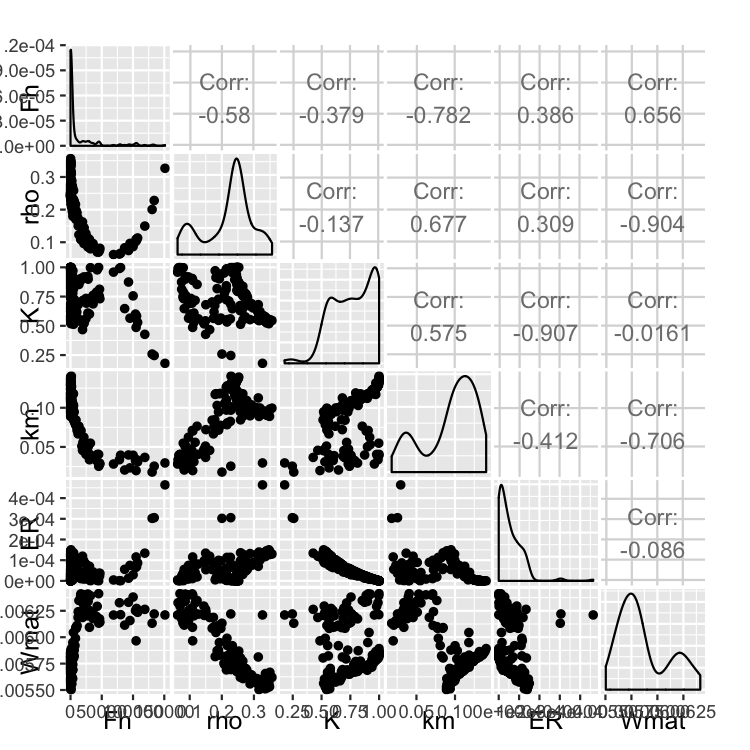
\includegraphics[width=\linewidth]{figure/Cat-fits-1-1} \hfill{}

\caption[Pairwise plot of parameter estimates from fitting Cat's growth and reproduction dataset]{Pairwise plot of parameter estimates from fitting Cat's growth and reproduction dataset.}\label{fig:Cat-fits-1}
\end{figure}


\end{knitrout}

Moreover, many of the ``consensus'' parameter estimates (in the sense that these estimates were very common) seem biologically unreasonable.
For example, all of the 25 best-fitting parameter sets have estimates of the half-saturation constant less than 500 cells/mL, which, given translates into 0.0036 mgC/L.
McCauley et al. 2008 used a half-saturation constant of 0.164 mgC/L, which is 50 times higher.
All of the 25 best-fitting parameter sets have estimates of $\kappa$ greater than 0.8, whereas McCauley et al. has an estimate of 0.23.

I think the best thing to do is to try fixing $F_h$ at different values, and see how that affects the other parameter estimates, since $F_h$  is specified by the feeding model, which was also ambiguous - relationships between parameters of the fitting model were highly constrained, but the parameter estimates themselves were highly flexible.
Although I doubt if there is a parameter set with a higher likelihood that was overlooked by the algorithm, my sense is that it may be that the likelihood surface is quite flat, so $f_h$ can run off towards 0, dragging all of the other parameter estimates with it.
The profile likelihood will be very informative in this regard.
I will also vary $v$, to see if that makes any difference to the fits, since that parameter is also fixed \emph{a priori}.

Fig. \ref{fig:Fh-profile} shows pretty clearly that many of the key parameters are dependent on the value of $F_h$.
In particular, the best estimates of both $\rho$ and $k_m$ decrease almost linearly with the fixed value of $F_h$.
$\kappa$, $E_R$, and $W_{mat}$, on the other hand, vary with $F_h$ when it is small, but as $F_h$ increases beyond approximately 10,000, the estimates remain fairly consistent.
Another obvious take-away from this plot is that $\kappa$ and $E_R$ are hard to estimate.

Basically, the take-away here is that there is very little information to fix either the value of $F_h$ or $v$, which I had already suspected.
Fortunately, there are plenty of other datasets that have estimated values of $F_h$ that I can use to fix the value of $F_h$ for these parameter estimations.
Nisbet et al. (2004) estimates $F_h = 0.08$ mgC/L for \emph{D. pulicaria}; McCauley et al. (1990) estimates $F_h = 0.16$ mgC/L; Hall et al. (2009) estimates $F_h = 0.1$ mgC/L for \emph{D. dentifera}; Martin et al. (2013) estimates $F_h = 1585$ cells/mL for \emph{D. magna};
Note that $F_h$ is measured here in units of cells/mL as well; the estimate of carbon context per cell is 8.16536$\times 10^{-9}$ mgC/cell.
If we use 0.1 mgC/L as the half-saturation constant (based on Hall et al.), that would be the equivalent of 0.1 mgC/L divided by 8.16536$\times 10^{-9}$ mgC/cell divided by 1000 mL/L = 12250 cells/mL, whereas if we use $0.16$ (based on McCauley et al. 1990, but also used by McCauley et al. 2008 and Johnson et al. 2013), the half-saturation constant would be 19,600 cells/mL.

Comparing the parameter estimates for $F_h = 12000$ and $F_h = 20000$,

\begin{tabular}{l | l | l}
& $F_h = 12000$ & $F_h = 20000$ \\
$\rho$ & 0.15 & 0.20 \\
$\kappa$ & 0.682 & 0.686 \\
$k_m$ & 0.073 & 0.054 \\
$E_R$ & $5.4 \times 10^{-5}$ & $4.8 \times 10^{-5}$ \\
$W_{mat}$ & $6.2 \times 10^{-3}$ & $6.3 \times 10^{-3}$ \\
$L_{obs}$ & 0.1 & 0.1 \\
$R_{obs}$ & 4.45 & 4.45 \\
loglik & 211 & 211
\end{tabular}

There are only very small differences between these two parameter sets, and no difference in the log-likelihood of either, indicating that they both are equally good at explaining the data.
The relationship between these parameter estimates and other published estimates is also useful.
For example, an estimate of $\kappa$ of 0.68 is \emph{very} different from the estimates of Nisbet et al. (2004).
Nisbet et al. (2004) fits a flexible spline to allocation fraction, showing that it drops from 1 to less than 0.2 very quickly.
McCauley et al. (2008) use an estimate of 0.23 (based on Nisbet).
Johnson et al. (2013) have estimates of $\kappa$ that vary quite considerably depending on the details of the model, from almost 0 when all parameters are left free, to between 0.3 and 0.7 when maximum size is constrained by an informative prior.
Martin et al. (2013) estimated $\kappa$ to be 0.678, which is very close to our estimate.
Thus, the estimate of $\kappa$ is reasonably well-supported, since Johnson et al. and Martin et al. both fit the standard DEB model to data, whereas Nisbet et al. was using a somewhat more bespoke model.

\begin{knitrout}\scriptsize
\definecolor{shadecolor}{rgb}{0.969, 0.969, 0.969}\color{fgcolor}\begin{figure}

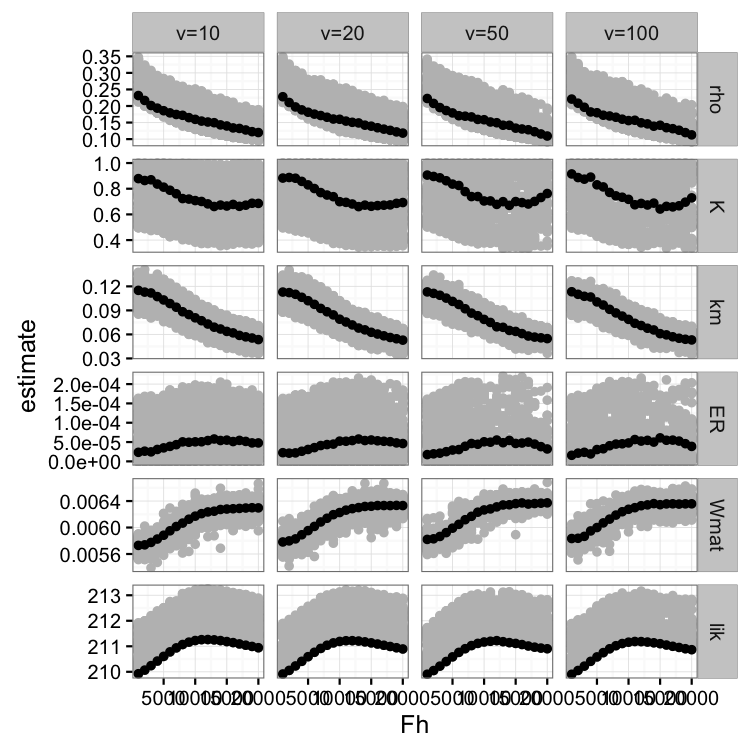
\includegraphics[width=\linewidth]{figure/Fh-profile-1} \hfill{}

\caption[Parameter estimates and likelihoods as the half-saturation constant and mobilization flux are varied]{Parameter estimates and likelihoods as the half-saturation constant and mobilization flux are varied.}\label{fig:Fh-profile}
\end{figure}


\end{knitrout}

We can compare the output of the model when $F_h$ was fixed at 12,000 cells/mL to the observed data to see how well we caputred the observed growth and reproduction data.
You can see in Fig. \ref{fig:model-data-comp} that the model does a pretty reasonable job of capturing the observed data.
On the basis of this, I will assume that I can proceed to fitting models that include parasitism.

\begin{knitrout}\scriptsize
\definecolor{shadecolor}{rgb}{0.969, 0.969, 0.969}\color{fgcolor}\begin{figure}

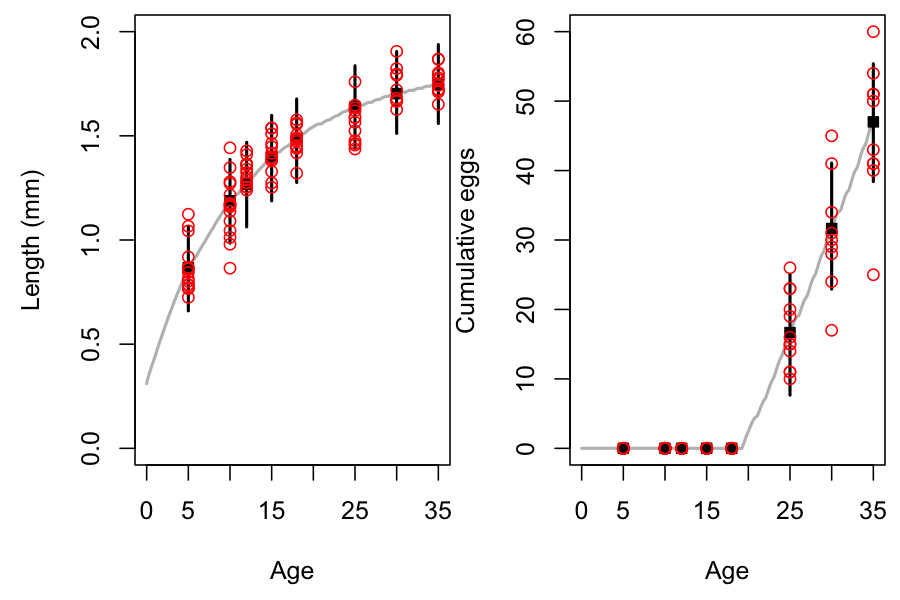
\includegraphics[width=\linewidth]{figure/model-data-comp-1} \hfill{}

\caption[Comparing model predictions to observed data]{Comparing model predictions to observed data. The gray line shows the deterministic prediction, and the black error bars show the model-predicted 95\% confidence interval at each age where data was observed. The red circles are observed data, which largely falls within the confidence interval, except for some of the reproduction data.}\label{fig:model-data-comp}
\end{figure}


\end{knitrout}

\section*{Infected animals}
For this, I really want to consider at least three possible models.
The first assumes that parasites use reserves as a resource, as in Hall et al. 2009.
The second assumes that parasites capture some fraction of the reserves that have been mobilized for growth.
The third assumes that parasites use soma as a resource.
I was somewhat ambiguous about which of models 2 and 3 I was actually considering in my Proc. B paper.

For the first model, the equation for parasite abundance is
\begin{equation}
\frac{dP}{dt} = e_P \frac{a_P E}{h_P + E} P - m P,
\end{equation}
where $e_P$ is the assimilation efficiency of the parasite, $a_P$ is the parasite's attack rate on reserves, $h_P$ is the parasite's half-saturation constant, and $m$ is the parasite's background mortality rate.

For the second model, the equation for parasite abundance is
\begin{equation}
\frac{dP}{dt} = e_P \frac{\phi_{max} P}{P_h + P} \kappa P_C - m P,
\end{equation}
where $\phi_{max}$ is the maximum fraction of growth allocation that the parasite population can capture, and $P_h$ is the half-saturation constant for parasite energy diversion.

For the first model, the equation for parasite abundance is
\begin{equation}
\frac{dP}{dt} = e_P \frac{a_P W}{h_P + W} P - m P,
\end{equation}
where $e_P$ is the assimilation efficiency of the parasite, $a_P$ is the parasite's attack rate on soma, $h_P$ is the parasite's half-saturation constant, and $m$ is the parasite's background mortality rate.



\end{document}
